\chapter{Results}
This chapter presents the result of the Blockchain in NDN experiment. The outcome of this experiment is interesting because it presents a different approach to verifying certificates. This project recognizes that, despite the apparent benefits of not having to contact the Certificate Authority for verification, there is also added complexity to the NDN security protocol. The results from this experiment investigate the trade off in this scenario, in different topologies using MiniNDN. Because of the serious time constraint imposed by our different modules, this project instead presents an ideal evaluation for the experiment.
\section{Ideal Evaluation}
Because of time constraints, only very limited testing was done with this project. The ideal evaluation for the Blockchain however, would involve testing a number of different realistic topologies. Ideally, one would request a certificate from the NDN team for the ability to test on the official testbed. This would allow for realistic results which are desirable. There are a number of different topologies that must be tested including the `dumbbell' topology with two chokepoint routers. It is desirable to test different data sets, with different data sizes, and also different intervals of node communication. There must be a control experiment for each of the listed experiments. MiniNDN allows for huge amounts of configuration and customization for each node in a topology. A user can set different Hyperbolic Routing variables as well as delay and bandwidth between nodes and also links, allowing for extensive and robust network testing.
\begin{figure}[ht]
\centering
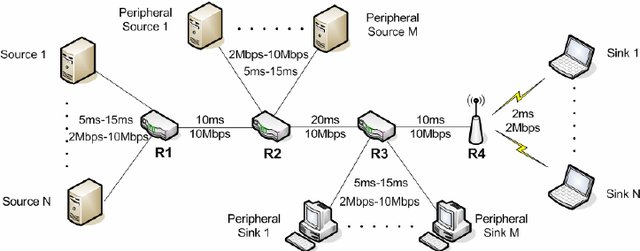
\includegraphics[scale=0.5]{topology.jpg}
\caption{Sample Topology \cite{057}}
\end{figure}

\begin{figure}
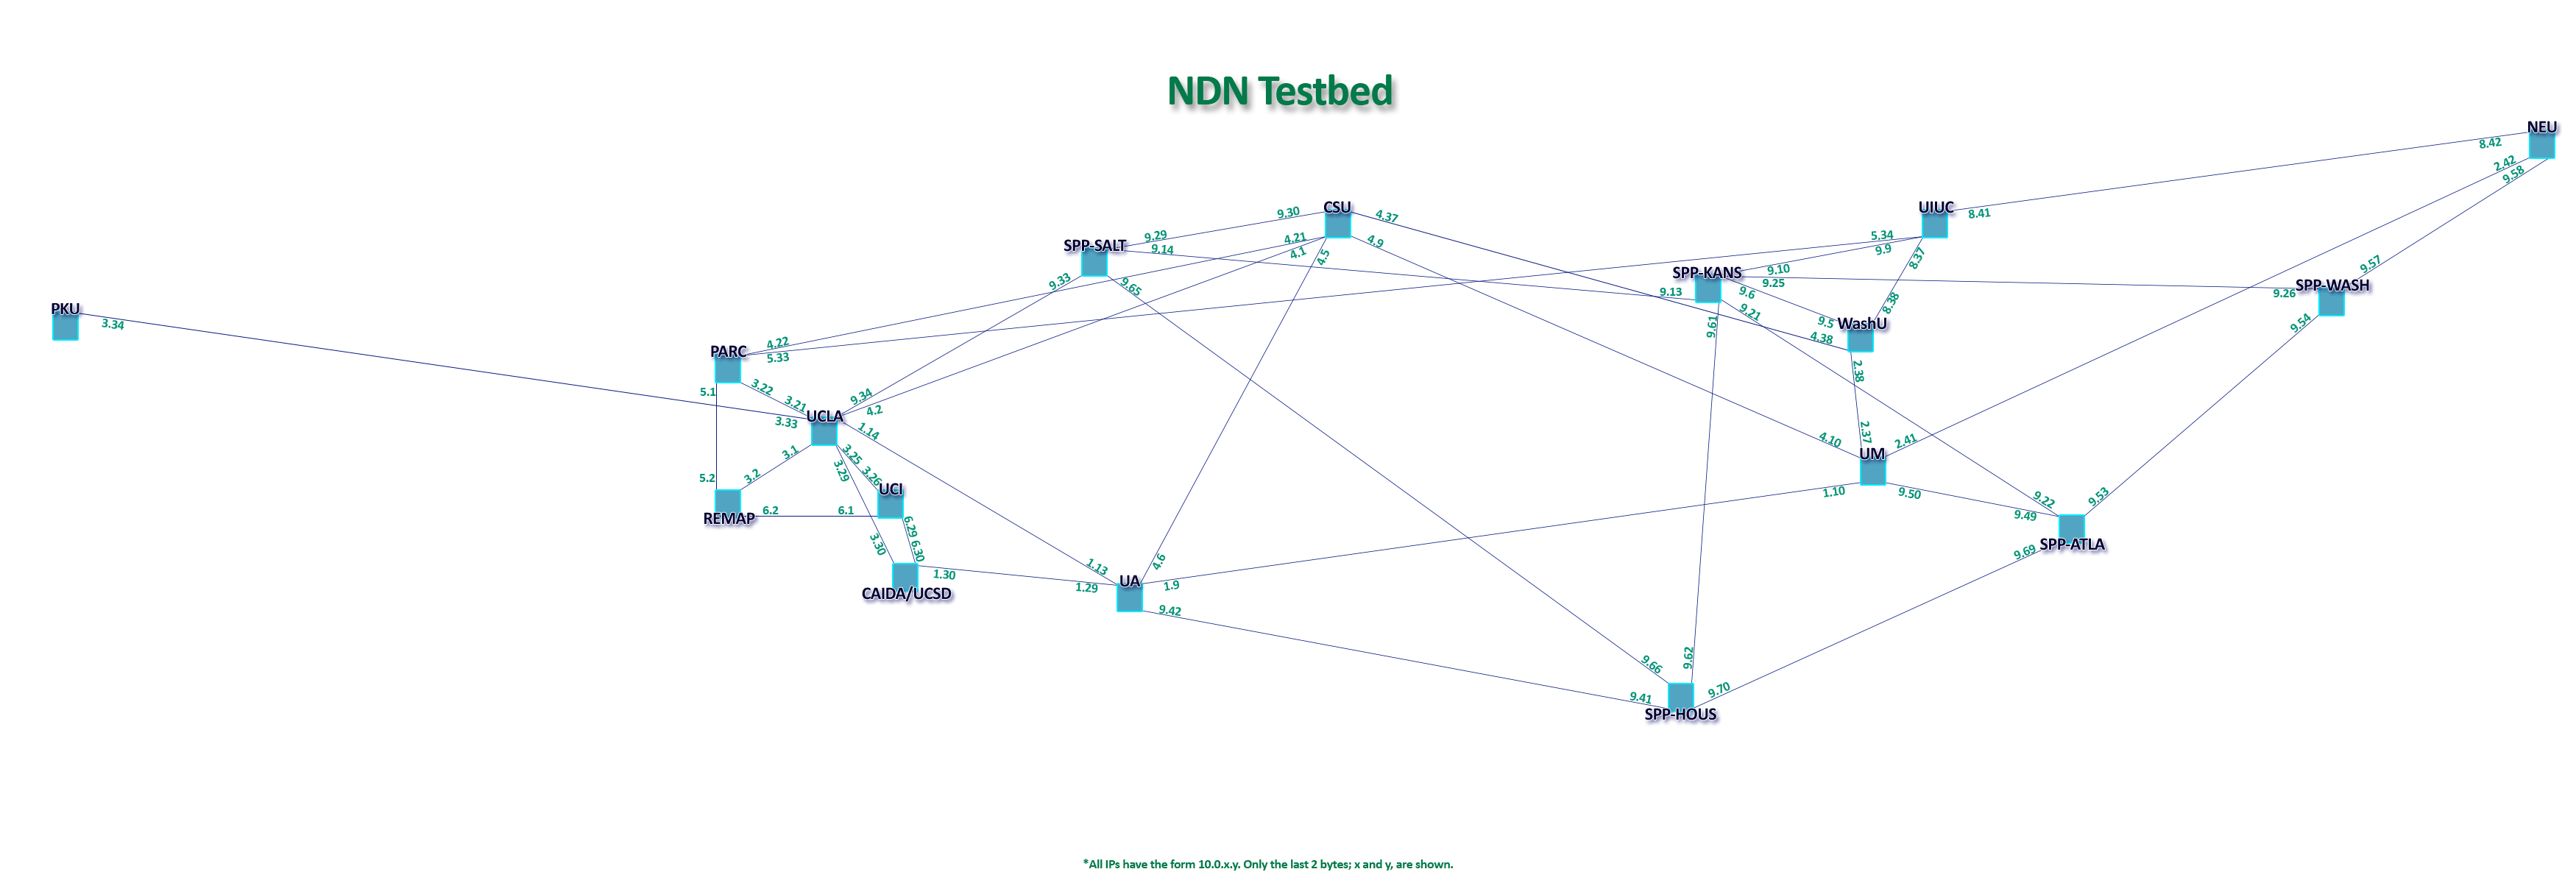
\includegraphics[width=6in]{topology.png}
\caption{The Current NDN Testbed Topology \cite{055}}
\end{figure}
\subsection{Overhead and Latency}
By increasing the complexity of NDN, one inadvertently adds overhead. The trade-off of that is the amount of time saved by nodes that don't have to communicate with the CA in order to verify Data. The concept itself works and isn't new. Browsers pre-install certificates to reduce look-up times. The idea here is to do the same by adding as little complexity as possible. And so, this project aims to achieve a golden ratio of complexity to efficiency. Adding the Blockchain data type to the NDN architecture adds bloat. If every node has that bit of overhead of having the Blockchain stored in its content store, it begs the question whether there's enough of a speed up from look-up reduction time to justify it. Especially seen as we are broadcasting the Blockchain, and some nodes might not be or want to be communicating at all. Yet, they are to request the Blockchain when the miners publish a Block.
\section{Discussion}
The evaluation of the success of this project greatly depends on whether one values a bigger Content Store or quicker communication between nodes. This is because every node would have to maintain the blocks in their cache. Blockchain in NDN greatly reduces communication with external Certificate Authorities. However, it can greatly add to the complexity of a network. Also, if it's a case of needing all nodes to have the Blockchain information simultaneously, then Chronosync is required, adding more complexity to the system. 
